% Style from https://stackoverflow.com/questions/1911516/how-to-make-cheat-sheets-in-latex/36768704#36768704
\documentclass[10pt,landscape,a4paper]{article}
\usepackage[utf8]{inputenc}
\usepackage[english]{babel}
\usepackage{amssymb}
\usepackage{amsmath}
\usepackage{tikz,pgf}
\usepackage{pgfplots}
\usetikzlibrary{angles,shapes,positioning,arrows,fit,calc,graphs,graphs.standard}
\usepackage{multicol}
\usepackage{wrapfig}
\usepackage[top=0mm,bottom=1mm,left=0mm,right=1mm]{geometry}
\usepackage[framemethod=tikz]{mdframed}
\usepackage{microtype}

\let\bar\overline

\DeclareMathOperator{\re}{Re}
\DeclareMathOperator{\im}{Im}
\DeclareMathOperator{\caparg}{Arg}
\DeclareMathOperator{\dom}{Dom}
\DeclareMathOperator{\codom}{Codom}
\DeclareMathOperator{\img}{Img}
\DeclareMathOperator{\Ind}{Ind}

\newcommand{\floor}[1]{\lfloor #1 \rfloor}      % simplifying the writing of a floor function
\newcommand{\ceiling}[1]{\lceil #1 \rceil}      % simplifying the writing of a ceiling function
\newcommand{\dotp}{\, \cdotp}             % dot product to distinguish from \cdot
\newcommand{\qed}{\hfill\ensuremath{\square}}   % Q.E.D sign
\newcommand{\abs}[1]{\left|#1\right|}           % absolute value
\newcommand{\at}[2]{\Big|_{#1}^{#2}}
\newcommand{\Arg}[1]{\caparg #1}
\renewcommand{\bar}[1]{\mkern 1.5mu \overline{\mkern -1.5mu #1 \mkern -1.5mu} \mkern 1.5mu}
\newcommand{\quotient}[2]{\faktor{#1}{#2}}
\newcommand{\cyclic}[1]{\left\langle #1 \right\rangle}
  % highlighting shortcuts
\newcommand{\hlimpo}[1]{\textcolor{base16-eighties-red}{\textbf{#1}}}
\newcommand{\hlwarn}[1]{\textcolor{base16-eighties-yellow}{\textbf{#1}}}
\newcommand{\hldefn}[1]{\textcolor{base16-eighties-blue}{\textbf{#1}}}
\newcommand{\hlnotea}[1]{\textcolor{base16-eighties-green}{\textbf{#1}}}
\newcommand{\hlnoteb}[1]{\textcolor{base16-eighties-lightblue}{\textbf{#1}}}
\newcommand{\hlnotec}[1]{\textcolor{base16-eighties-brown}{\textbf{#1}}}
\newcommand{\WTP}{\textcolor{base16-eighties-brown}{WTP}}
\newcommand{\WTS}{\textcolor{base16-eighties-brown}{WTS}}
\newcommand{\ind}[2]{\Ind_{#2}(#1)}
\renewcommand{\epsilon}{\varepsilon}
\newcommand*\dif{\mathop{}\!d}

\pgfplotsset{compat=1.15}
\usepgfplotslibrary{fillbetween}
\pgfplotsset{four quads/.append style={axis x line=middle, axis y line=
middle, xlabel={$x$}, ylabel={$y$}, axis equal }}
\pgfplotsset{four quad complex/.append style={axis x line=middle, axis y line=
middle, xlabel={$\re$}, ylabel={$\im$}, axis equal }}

\definecolor{myblue}{cmyk}{1,.72,0,.38}

\def\firstcircle{(0,0) circle (1.5cm)}
\def\secondcircle{(0:2cm) circle (1.5cm)}

\colorlet{circle edge}{myblue}
\colorlet{circle area}{myblue!5}

\tikzset{filled/.style={fill=circle area, draw=circle edge, thick},
    outline/.style={draw=circle edge, thick}}

\pgfdeclarelayer{background}
\pgfsetlayers{background,main}

\everymath\expandafter{\the\everymath \color{myblue}}
\everydisplay\expandafter{\the\everydisplay \color{myblue}}

\renewcommand{\baselinestretch}{.8}
\pagestyle{empty}

\global\mdfdefinestyle{header}{%
linecolor=gray,linewidth=1pt,%
leftmargin=0mm,rightmargin=0mm,skipbelow=0mm,skipabove=0mm,
}

\newcommand{\header}{
\begin{mdframed}[style=header]
\footnotesize
\sffamily
PMATH352W18 Cheatsheet\\
by~Johnson~Ng,~page~\thepage~of~1
\end{mdframed}
}

\makeatletter
\renewcommand{\section}{\@startsection{section}{1}{0mm}%
                                {.2ex}%
                                {.2ex}%x
                                {\color{myblue}\sffamily\small\bfseries}}
\renewcommand{\subsection}{\@startsection{subsection}{1}{0mm}%
                                {.2ex}%
                                {.2ex}%x
                                {\sffamily\bfseries}}



\def\multi@column@out{%
   \ifnum\outputpenalty <-\@M
   \speci@ls \else
   \ifvoid\colbreak@box\else
     \mult@info\@ne{Re-adding forced
               break(s) for splitting}%
     \setbox\@cclv\vbox{%
        \unvbox\colbreak@box
        \penalty-\@Mv\unvbox\@cclv}%
   \fi
   \splittopskip\topskip
   \splitmaxdepth\maxdepth
   \dimen@\@colroom
   \divide\skip\footins\col@number
   \ifvoid\footins \else
      \leave@mult@footins
   \fi
   \let\ifshr@kingsaved\ifshr@king
   \ifvbox \@kludgeins
     \advance \dimen@ -\ht\@kludgeins
     \ifdim \wd\@kludgeins>\z@
        \shr@nkingtrue
     \fi
   \fi
   \process@cols\mult@gfirstbox{%
%%%%% START CHANGE
\ifnum\count@=\numexpr\mult@rightbox+2\relax
          \setbox\count@\vsplit\@cclv to \dimexpr \dimen@-1cm\relax
\setbox\count@\vbox to \dimen@{\vbox to 1cm{\header}\unvbox\count@\vss}%
\else
      \setbox\count@\vsplit\@cclv to \dimen@
\fi
%%%%% END CHANGE
            \set@keptmarks
            \setbox\count@
                 \vbox to\dimen@
                  {\unvbox\count@
                   \remove@discardable@items
                   \ifshr@nking\vfill\fi}%
           }%
   \setbox\mult@rightbox
       \vsplit\@cclv to\dimen@
   \set@keptmarks
   \setbox\mult@rightbox\vbox to\dimen@
          {\unvbox\mult@rightbox
           \remove@discardable@items
           \ifshr@nking\vfill\fi}%
   \let\ifshr@king\ifshr@kingsaved
   \ifvoid\@cclv \else
       \unvbox\@cclv
       \ifnum\outputpenalty=\@M
       \else
          \penalty\outputpenalty
       \fi
       \ifvoid\footins\else
         \PackageWarning{multicol}%
          {I moved some lines to
           the next page.\MessageBreak
           Footnotes on page
           \thepage\space might be wrong}%
       \fi
       \ifnum \c@tracingmulticols>\thr@@
                    \hrule\allowbreak \fi
   \fi
   \ifx\@empty\kept@firstmark
      \let\firstmark\kept@topmark
      \let\botmark\kept@topmark
   \else
      \let\firstmark\kept@firstmark
      \let\botmark\kept@botmark
   \fi
   \let\topmark\kept@topmark
   \mult@info\tw@
        {Use kept top mark:\MessageBreak
          \meaning\kept@topmark
         \MessageBreak
         Use kept first mark:\MessageBreak
          \meaning\kept@firstmark
        \MessageBreak
         Use kept bot mark:\MessageBreak
          \meaning\kept@botmark
        \MessageBreak
         Produce first mark:\MessageBreak
          \meaning\firstmark
        \MessageBreak
        Produce bot mark:\MessageBreak
          \meaning\botmark
         \@gobbletwo}%
   \setbox\@cclv\vbox{\unvbox\partial@page
                      \page@sofar}%
   \@makecol\@outputpage
     \global\let\kept@topmark\botmark
     \global\let\kept@firstmark\@empty
     \global\let\kept@botmark\@empty
     \mult@info\tw@
        {(Re)Init top mark:\MessageBreak
         \meaning\kept@topmark
         \@gobbletwo}%
   \global\@colroom\@colht
   \global \@mparbottom \z@
   \process@deferreds
   \@whilesw\if@fcolmade\fi{\@outputpage
      \global\@colroom\@colht
      \process@deferreds}%
   \mult@info\@ne
     {Colroom:\MessageBreak
      \the\@colht\space
              after float space removed
              = \the\@colroom \@gobble}%
    \set@mult@vsize \global
  \fi}

\makeatother
\setlength{\parindent}{0pt}

\begin{document}
\small
\begin{multicols*}{5}
\section{Complex Numbers and Their Properties}
\subsection*{Complex Plane as a Set}
$\mathbb{C} = \mathbb{R}^2 = \left\{\begin{pmatrix} x \\ y \end{pmatrix} : x, y \in \mathbb{R} \right\}$
\subsection*{Real and Imaginary Part}
$\forall z = x + iy \in \mathbb{C} \; x, y \in \mathbb{R} \\ \re(z) = x \; \im(z) = y$
\subsection*{Product}
$\forall z = a + ib, w = c + id \in \mathbb{C} \; a, b, c, d \in \mathbb{R} \\
zw = (ac - bd) + i (ad + bc)$
\subsection*{Inverse of a Complex Number}
$\forall z = a + ib \in \mathbb{C} \; a, b \in \mathbb{R} \\
\exists z^{-1} = \frac{a}{aa^2 + b^2} - i \frac{b}{a^2 + b^2} \in \mathbb{C}$
\subsection*{Conjugate}
$\forall z = a + ib \in \mathbb{C} \; a, b \in \mathbb{R} \\
\exists \bar{z} = a - ib \in \mathbb{C}$
\subsection*{Modulus}
$\forall z = x = iy \in \mathbb{C} \; x, y \in \mathbb{R} \\
\abs{z} = \sqrt{x^2 + y^2} \in \mathbb{R}$
\subsection*{Basic Inequalities}
$\forall z, w \in \mathbb{C},$
\begin{enumerate}
	\item $\abs{\re(z)} \leq \abs{z}$
	\item $\abs{\im(z)} \leq \abs{z}$
	\item $\abs{z + w} \leq \abs{z} + \abs{w}$
	\item $\abs{z + w} \geq \abs{ \; \abs{z} + \abs{w} \; }$
\end{enumerate}
\subsection*{Region of a set of Complex Numbers}
Describe $\{z \in \mathbb{C} : \abs{z - a} < \abs{z - b}\}$.
\resizebox{\columnwidth}{!}{
	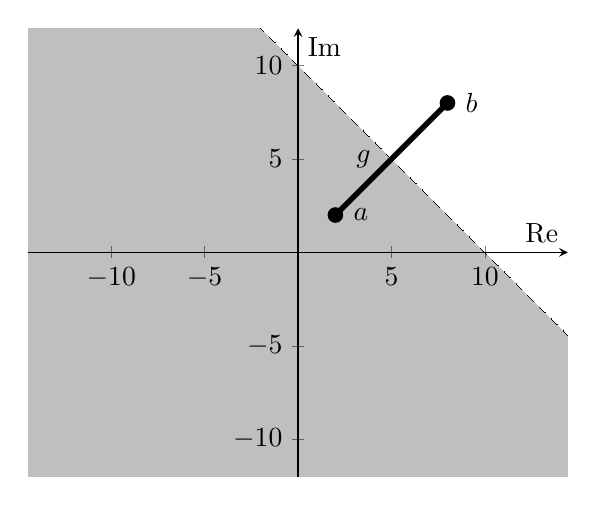
\begin{tikzpicture}
		\begin{axis}[four quad complex, xmin=-12, xmax=12, ymin=-12, ymax=12]
			\draw[line width=0pt,dashed,fill=black,fill opacity=0.25](-20,20)--(-20,-20)--(20,-20)--(20,-10)--(-5,15);
			\draw[color=black] (-1,13) node {$f$};
			\draw[line width=2pt,solid](2,2)--(8,8);
			\draw[color=black] (3.5,5) node {$g$};
			\node[label={0:{$a$}},circle,fill,inner sep=2pt] at (axis cs:2,2) {};
			\node[label={0:{$b$}},circle,fill,inner sep=2pt] at (axis cs:8,8) {};
		\end{axis}
	\end{tikzpicture}
}
\subsection*{Every complex number has exactly 2 roots}
$\forall z = x = iy \in \mathbb{C} \; x, y \in \mathbb{R} \\
\exists w_{1, 2} = u + iv \in \mathbb{C} \; u, v \in \mathbb{R}$
\begin{equation*}
	\resizebox{\columnwidth}{!}{%
		$w = \begin{cases}
			\pm \left[ \left(\frac{x + \sqrt{x^2 + y^2}}{2} \right)^{\frac{1}{2}} + i \left( \frac{-x + \sqrt{x^2 + y^2}}{2} \right)^{\frac{1}{2}} \right] & y > 0 \\
			\pm \left[ \left(\frac{x + \sqrt{x^2 + y^2}}{2} \right)^{\frac{1}{2}} - i \left(\frac{-x + \sqrt{x^2 + y^2}}{2} \right)^{\frac{1}{2}} \right] & y < 0 \\
			\pm \sqrt{x} & y = 0, x > 0 \\
			\pm i \sqrt{x} & y = 0, x < 0
		\end{cases}$
	}
\end{equation*}
\subsection*{Quadratic Formula}
$\forall a, b, c \in \mathbb{C} \; a \neq 0 \; az^2 + bz + c = 0$
\begin{equation*}
	z = \frac{-b + \sqrt{b^2 - 4ac}}{2a}
\end{equation*}
\subsection*{Argument}
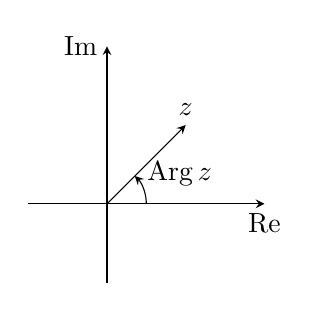
\begin{tikzpicture}
	\tikzset{>=stealth}
	\draw[->] (-1, 0) -- ++(3, 0) coordinate (X) node[below] {$\re$};
	\draw[->] (0, -1) -- ++(0, 3) node[left] {$\im$};
	\coordinate (O) at (0, 0);

	\draw[->] (O) -- (1,1) coordinate (z) node[above] {$z$};
	\path (X) -- (O) -- (z) pic [draw,->,pic text=$\Arg{z}$, angle eccentricity=2.0] {angle=X--O--z};
\end{tikzpicture}
\subsection*{Polar Form}
$\forall z \in \mathbb{C} \; \exists r, \theta \in \mathbb{R} \; \theta \in [0, 2\pi)$ \\
$z = re^{i\theta}$
\subsection*{Polar to Cartesian}
$x = r \cos \theta \quad y = r \sin \theta$
\subsection*{Cartesian to Polar}
$r = \abs{z} \quad \tan \theta = \frac{x}{y}$
\subsection*{Conjugate in Polar Form}
$z = re^{i\theta} \iff \bar{z} = re^{-i\theta}$
\subsection*{Inverse in Polar Form}
$z = re^{i \theta} \land z \neq 0 \\
\implies z^{-1} = \frac{1}{r} e^{-i \theta}$
\subsection*{Product in Polar Form}
\begin{itemize}
	\item $z_1 z_2 = r_1 r_2 e^{i (\theta_1 + \theta_2)}$
	\item $\forall n \in \mathbb{Z} \enspace (re^{in}) = r^n e^{in\theta}$
\end{itemize}
\subsection*{nth Roots of a Complex Number}
$\left\{ r^{\frac{1}{n}} e^{i \left(\frac{\theta + 2 \pi k}{n} \right)} : k = 0, 1, ..., n - 1 \right\}$
\subsection*{nth Roots of Unity}
$\left\{ e^{i \left(\frac{2 \pi k}{n} \right)} : k = 0, 1, ..., n - 1 \right\}$

\section{Complex Functions} % (fold)
\label{sec:complex_functions}

\subsection{Convergence} % (fold)
\label{sub:convergence}
$\forall \{z_n\}_{n \in \mathbb{N}} \subseteq \mathbb{C} \enspace \land \enspace z \in \mathbb{Z} \\
	(n \to \infty \implies z_n \to z) \iff \lim_{n \to \infty} \abs{z_n - z} = 0$

May also write as $\lim_{n \to \infty} z_n = z$
% subsection convergence (end)

\subsection{Convergence for Complex Functions} % (fold)
\label{sub:convergence_for_complex_functions}
$\forall \Omega \subseteq \mathbb{C} \enspace \forall f : \Omega \to \mathbb{C} \enspace z_0 \in \mathbb{C} \enspace \exists L \in \mathbb{C} \enspace \forall \{z_n\}_{n \in \mathbb{N}} \subseteq \Omega \setminus \{z_0\}$

$(z_n \to z_0 \implies f(z_0) \to L) \implies \lim_{z \to z_0} f(z) = L$
% subsection convergence_for_complex_functions (end)

\subsection{Continuity} % (fold)
\label{sub:continuity}

$\forall f : \Omega \subseteq \mathbb{C} \to \mathbb{C}$

$f$ is continuous on $z_0 \implies$
\begin{enumerate}
	\item $\forall \{z_0\}_{n \in \mathbb{N}} \enspace z_n \to z_0 \implies f(z_n) \to f(z_0)$
	\item $\forall z \in \Omega \; \forall \epsilon > 0 \; \exists \delta > 0 \enspace \abs{z - z_0} < \delta \implies \abs{f(z) - f(z_0)} < \epsilon$
\end{enumerate}

% subsection continuity (end)

\subsection{Real and Imaginary Parts of a Function} % (fold)
\label{sub:real_and_imaginary_parts_of_a_function}

$f(z) = u(x, y) + iv(x, y)$

% subsection real_and_imaginary_parts_of_a_function (end)

% section complex_functions (end)
\section{Differentiation} % (fold)
\label{sec:differentiation}

\subsection{Neighbourhood} % (fold)
\label{sub:neighbourhood}

$\forall z_0 \in \mathbb{C} \; r \in \mathbb{R} \; D(z_0, r) := \{z in \mathbb{C} : \abs{z - z_0} < r\}$ is the neighbourhood of radius $r$ around $z_0$.

% subsection neighbourhood (end)

\subsection{Differentiation/Holomorphic} % (fold)
\label{sub:differentiation_holomorphic}

Let $z_0 \in \mathbb{C} \; r \in \mathbb{R} \; \exists D(z_0, r) \subseteq \mathbb{R}$. $\forall f : D(z_0, r) \to \mathbb{C} \; \forall h \in \mathbb{C}$

$\exists \lim_{h \to 0} \frac{f(z_0 + h) - f(z_0)}{h} \implies$ $f$ is differentiable/holomorphic $\land \; f'(z_0) = \lim_{h \to 0} \frac{f(z_0 + h) - f(z_0)}{h}$

% subsection differentiation_holomorphic (end)

\subsection{Properties of Holomorphic Functions} % (fold)
\label{sub:properties_of_holomorphic_functions}
$f, g$ are holomorphic at $z \in \mathbb{C} \implies$
\begin{enumerate}
	\item $(f + g)' = f' + g'$
	\item $(fg)' = f'g + fg'$
	\item $(g \neq 0 \implies (\frac{f}{g})' = \frac{f'g - fg'}{g^2} )$
\end{enumerate}

% subsection properties_of_holomorphic_functions (end)

\subsection{Cauchy-Riemann Equations} % (fold)
\label{sub:cauchy_riemann_equations}

$\forall z_0 = x_0 + iy_0 \in \mathbb{C} \; x_o, y_o \in \mathbb{R}$. $f(z)$ is holomorphic at $z_0 \implies$ at $(x_0, y_0)$
\begin{equation*}
	\frac{\partial u}{\partial x} = \frac{\partial v}{\partial y} \; \land \; \frac{\partial v}{\partial x} = - \frac{\partial u}{\partial y}  
\end{equation*}

% subsection cauchy_riemann_equations (end)

\subsection{Conditional Converse of CRE} % (fold)
\label{sub:conditional_converse_of_cre}
Let $z_0 = z_0 + iy_0 \in \mathbb{\Omega} \subseteq \mathbb{R} \; x_0, y_0 \in \mathbb{R} \; u, v : \mathbb{R^2} \to \mathbb{R} \; f = u + iv : \Omega \to \mathbb{C}$.
\begin{enumerate}
	\item partials of $u, v$ exist in nbd of $x_0, y_0)$
	\item partials of $u, v$ are cont' at $(x_0, y_0)$
	\item $\frac{\partial u}{\partial x} = \frac{\partial v}{\partial y} \; \land \; \frac{\partial v}{\partial x} = - \frac{\partial u}{\partial y}  $
\end{enumerate}
$\implies f$ is holo at $z_0$.

% subsection conditional_converse_of_cre (end)

\subsection{Power Series} % (fold)
\label{sub:power_series}

Infinite series of the form $\sum_{n \in \mathbb{N}} c_n z^n$

% subsection power_series (end)

\subsection{Convergence for Power Series} % (fold)
\label{sub:convergence_for_power_series}

We will usually aim for absolute convergence, for

\begin{equation*}
	\abs{\sum_{n=0}^{N} c_n z^n} \leq \sum_{n=0}^{N} \abs{c_n} \abs{z}^n
\end{equation*}

% subsection convergence_for_power_series (end)

\subsection{Hadamard's Formula} % (fold)
\label{sub:hadamard_s_formula}

$\frac{1}{R} := \limsup_{n \to \infty} \abs{c_n}^\frac{1}{n}$.

% subsection hadamard_s_formula (end)

\subsection{Limit Supremum} % (fold)
\label{sub:limit_supremum}
\begin{equation*}
	\limsup_{n \to \infty} a_n := \lim_{n \to \infty} \sup_{m \geq n} a_m
\end{equation*}
% subsection limit_supremum (end)

\subsection{limsup Property} % (fold)
\label{sub:limsup_property}
$\forall \{a_n\}_{n \in \mathbb{N}} L:=\limsup_{n \to \infty} a_n \implies$

$\forall \epsilon > 0 \; \exists N > 0 \; \forall n > N$

$\abs{a_0 - L} < \epsilon$

% subsection limsup_property (end)

\subsection{Radius of Convergence} % (fold)
\label{sub:radius_of_convergence}
$\forall \sum_{n \in \mathbb{N}} c_n z^n \; \exists 0 \leq R < \infty$
\begin{enumerate}
	\item $\abs{z} < R \implies$ absolute convergence
	\item $\abs{z} > R \implies$ divergence
\end{enumerate}
% subsection radius_of_convergence (end)

\subsection{Power Function and its Holomorphic Function share the same Region of Convergence} % (fold)
\label{sub:power_function_and_its_holomorphic_function_share_the_same_region_of_convergence}

$f(z) = \sum_{n \in \mathbb{N}} c_n z^n $ had a rad of conv $R \in \mathbb{R} \implies \forall \{z : \abs{z} < R\}$

\begin{equation*}
	f'(z) = \sum_{n=1}^{\infty} nc_n z^{n - 1}
\end{equation*}

rad of conv of $f'$ is $R$.

% subsection power_function_and_its_holomorphic_function_share_the_same_region_of_convergence (end)

\subsection{Entire Function} % (fold)
\label{sub:entire_function}
$f$ is said to be entire if $f$ is holomorphic in the entire $\mathbb{C}$.
% subsection entire_function (end)

% section differentiation (end)
\section{Integration} % (fold)
\label{sec:integration}

\subsection{Curves} % (fold)
\label{sub:curves}
A curve in $\mathbb{C}$ is a cont' fn $\gamma : [a, b] \subseteq \mathbb{R} \to \mathbb{C}$. Image of $\gamma$ is called $\gamma^*$.
% subsection curves (end)

\subsection{Equivalent Parameterization} % (fold)
\label{sub:equivalent_parameterization}
Let $\gamma_1 : [a, b] \subseteq \mathbb{R} \to \mathbb{C} \; \gamma_2 : [c, d] \subseteq \mathbb{R} \to \mathbb{C}$ desc path $\gamma^*$. $\gamma_1, \gamma_2$ are equiv if $\exists h : [a, b] \to [c, d]$, bijective and cont', s.t. $\forall t \in \dom(h) \; \gamma_1 (t) = \gamma_2(h(t))$.
% subsection equivalent_parameterization (end)

\subsection{Smooth Curve} % (fold)
\label{sub:smooth_curve}
$\gamma$ is smooth if $\exists \gamma'$ is cont' on $\dom(\gamma) \; \land \; \forall t \in \dom(\gamma) \; \gamma'(t) \neq 0$.
% subsection smooth_curve (end)

\subsection{Piecewise Smooth Curve} % (fold)
\label{sub:piecewise_smooth_curve}
$\gamma$ is piecewise smooth if $\gamma$ is smooth on $\dom(\gamma)$ except on finitely many pts.
% subsection piecewise_smooth_curve (end)

\subsection{Integral over path} % (fold)
\label{sub:integral_over_path}
Let $\gamma: [a, b] \to \mathbb{C} \; \land \; f : \mathbb{C} \to \mathbb{C}$ con' on $\gamma$. Integral $f$ along $\gamma$ is
\begin{equation*}
	\int_{\gamma} f(z) dz = \int_{a}^{b} f(\gamma(t))\gamma'(t) dt
\end{equation*}
Integral over a curve $\gamma^*$ is independent of the path chosen.
% subsection integral_over_path (end)

\subsection{Integral Properties} % (fold)
\label{sub:integral_properties}
\begin{enumerate}
	\item (Linearity) $\int_{\gamma} (\alpha f + \beta g) = \alpha \int_{\gamma} f + \beta \int_{\gamma} g$
	\item \begin{enumerate}
		\item $\abs{\int_{a}^{b} g} \leq \int_{a}^{b} \abs{g}$
		\item $\abs{\int_{\gamma} f dz} \leq \sup_{z \in \Omega} f(z) \cdot \int_{a}^{b} \abs{\gamma'(t)} dt$
	\end{enumerate}
	\item $\gamma^-$ is in opposite orientation of $\gamma \implies \int_{\gamma^-} f = - \int_{\gamma} f$
\end{enumerate}
% subsection integral_properties (end)

\subsection{Fundamental Theorem of Calculus} % (fold)
\label{sub:fundamental_theorem_of_calculus}
Let $(\gamma : [a, b] \subseteq \mathbb{R} \to \mathbb{C}) \in \Omega \subseteq \mathbb{C}$. $f$ cont' on $\gamma \; \exists F' = f$ holo on $\Omega \implies \int_{\gamma} f = F(\gamma(b)) - F(\gamma(a))$
% subsection fundamental_theorem_of_calculus (end)

\subsection{Corollary of FTC} % (fold)
\label{sub:corollary_of_ftc}
If $F \in H(\Omega), \, \Omega \subseteq \mathbb{C}, \, \gamma \subseteq \Omega$ that is a closed path, then
\begin{equation*}
	\int_{\gamma} F'(z) \dif{z} = 0
\end{equation*}
% subsection corollary_of_ftc (end)

\subsection{Goursat's Theorem} % (fold)
\label{sub:goursat_s_theorem}
Let $\Omega \subseteq \mathbb{C}$ be open. Sps $\Delta \subseteq \Omega$ is a closed triangle, and $\Delta^0 \subseteq \Omega$, and let $f \in H(\Omega)$. Then
\begin{equation*}
	\int_{\Delta} f(z) \dif{z} = 0
\end{equation*}
% subsection goursat_s_theorem (end)

\subsection{Convex Set} % (fold)
\label{sub:convex_set}
A set $S \subseteq \mathbb{C}$ is a convex set if the line segment joining any pair of points in $S$ lies entirely in $S$.
% subsection convex_set (end)

\subsection{Cauchy's Theorem for Convex Set} % (fold)
\label{sub:cauchy_s_theorem_for_convex_set}
Let $\Omega \subseteq \mathbb{C}$ be a convex open set, and $f \in H(\Omega)$. Then
\begin{enumerate}
	\item $f = F'$ for some $F \in H(\Omega)$
	\item $\int_{\gamma} f(z) \dif{z} = 0$ for any closed path $\gamma \in \Omega$
\end{enumerate}
% subsection cauchy_s_theorem_for_convex_set (end)

\subsection{Cauchy's Integral Formula 1} % (fold)
\label{sub:cauchy_s_integral_formula_1}
Let $\Omega \subseteq \mathbb{C}$ be a convex open set, and $C$ be a closed circle path in $\Omega$. If $w \in \Omega \setminus \partial C$, and $f \in H(\Omega)$, then
\begin{equation*}
	f(w) \ind{w}{C} = \frac{1}{2 \pi i} \int_{C} \frac{f(z)}{z - w} \dif{z}
\end{equation*}
where
\begin{equation*}
	\ind{w}{C} = \frac{1}{2 \pi i} \int_{\gamma} \frac{\dif{z}}{z - w}
\end{equation*}
% subsection cauchy_s_integral_formula_1 (end)

\subsection{Holomorphic Functions as Power Series} % (fold)
\label{sub:holomorphic_functions_as_power_series}
Let $\Omega \subseteq \mathbb{C}$ be an open set, $f \in H(\Omega)$. Then $f$ can be expressed as a power series.
% subsection holomorphic_functions_as_power_series (end)

\subsection{Cauchy's Integral Formula 2} % (fold)
\label{sub:cauchy_s_integral_formula_2}
Let $\Omega \subseteq \mathbb{C}$ be open, $f \in H(\Omega)$. Then
\begin{enumerate}
	\item $\forall w \in \Omega, \, f$ has a power series expansion at $w$
	\item $f$ is differentiable infinitely many times in $\Omega$
	\item $\forall C \subseteq \Omega$ that is a closed circle oriented anticlockwise, $\forall w \in C^0$,
	\begin{equation*}
		f^{(n)}(w) = \frac{n!}{2 \pi i} \int_{C} \frac{f(z)}{(z - w)^{n + 1}} \dif{z}
	\end{equation*}
\end{enumerate}
% subsection cauchy_s_integral_formula_2 (end)

\subsection{Taylor Expansion of Entire Functions} % (fold)
\label{sub:taylor_expansion_of_entire_functions}
If $f$ is entire, then $\forall z_0 \in \mathbb{C}$,
\begin{equation*}
	f(z) = \sum_{n=0}^{\infty} \frac{f^{(n)}(z_0)}{n!} (z - z_))^n
\end{equation*}
% subsection taylor_expansion_of_entire_functions (end)

\subsection{Analytic Functions} % (fold)
\label{sub:analytic_functions}
$f$ is analytic in $\Omega$ if $f$ has a power series expansion $\forall z \in \Omega$.
% subsection analytic_functions (end)

\subsection{Analyticity \& Holomorphicity} % (fold)
\label{sub:analyticity_&_holomorphicity}
It is an iff relation
% subsection analyticity_&_holomorphicity (end)

\subsection{Cauchy's Inequality} % (fold)
\label{sub:cauchy_s_inequality}
$\forall z_0 \in \mathbb{C} \; \forall R > 0 \in \mathbb{R} \; \forall f \in H(C = D(z_0, R))$
\begin{equation*}
	f^{(n)}(z_0) \leq \frac{n!}{R^n} \cdot \sup_{z \in C} \abs{f(z)}
\end{equation*}
% subsection cauchy_s_inequality (end)

\subsection{Liouville's Theorem} % (fold)
\label{sub:liouville_s_theorem}
A bounded entire function $f : \mathbb{C} \to \mathbb{C}$ is a constant.
% subsection liouville_s_theorem (end)

\subsection{Parseveal's Theorem} % (fold)
\label{sub:parseveal_s_theorem}
$\Omega \subseteq \mathbb{C}$ be open, $f \in H(\Omega)$, $\bar{D(z_0, R)} \subseteq \Omega \implies$

$\forall z \in \bar{D(z_0, R)}, \, f(z) = \sum_{n=0}^{\infty} c_n (z - z_0)^n \implies$

$\forall z \in \bar{D(z_0, R)} \enspace f(z_0 + re^{i \theta}) = \sum_{n=0}^{\infty} c_n (re^{i \theta})^n$
% subsection parseveal_s_theorem (end)

\subsection{Parseval's Indentity} % (fold)
\label{sub:parseval_s_indentity}
Same setup as above,
\begin{equation*}
	\frac{1}{2 \pi} \int_{0}^{2 \pi} \abs{f(z_0 = re^{i \theta})}^2 \dif{\theta} = \sum_{n=0}^{\infty} \abs{c_n}^2 r^{2n}
\end{equation*}
% subsection parseval_s_indentity (end)

\subsection{Principle of Analytic Continuation} % (fold)
\label{sub:principle_of_analytic_continuation}
$\Omega \subseteq \mathbb{C}$ open \& connected, $f \in H(\Omega)$. $Z(f) := \{a \in \Omega : f(a) = 0 \}$. Then either $Z(f) = \Omega$ or $Z(f)$ has no limit point (i.e. points where $f = 0$ are isolated)
% subsection principle_of_analytic_continuation (end)

\subsection{Maximum Modulus Principle} % (fold)
\label{sub:maximum_modulus_principle}

$\Omega \subseteq \mathbb{C} \, f \in H(\Omega) \, \exists r > 0 \, D_{z_0} = \bar{D(z_0, r)} \subseteq \Omega \implies$

$\abs{f(z_0)} \leq \max_{z \in \partial D_{z_0}} \abs{f(z)}$ and

$\abs{f(z_0)} = \max_{z \in \partial D_{z_0}} \iff f $ is constant on $\Omega$

% subsection maximum_modulus_principle (end)

\subsection{Fundamental Theorem of Algebra} % (fold)
\label{sub:fundamental_theorem_of_algebra}
$\forall P(z) \in \mathbb{C}[z] \, \deg P(z) = n \in \mathbb{N} \, \exists \alpha_1, \alpha_2, ..., \alpha_n \in \mathbb{C} \, \land \exists A \in \mathbb{C}$
\begin{equation*}
	P(z) = A(z - \alpha_1)(z - \alpha_2) \hdots (z - \alpha_n)
\end{equation*}
% subsection fundamental_theorem_of_algebra (end)

\subsection{Uniqueness of a Function} % (fold)
\label{sub:uniqueness_of_a_function}
$\Omega \subseteq \mathbb{C}$ open \& connected, $\forall f, g \in H(\Omega)$

For any $\Omega' \subseteq \Omega$, $\forall z \in \Omega' \; f(z) = g(z) \implies$

$\forall z \in \Omega \; f(z) = g(z)$
% subsection uniqueness_of_a_function (end)

% section integration (end)

\end{multicols*}
\end{document}